
%% Introduction


\section{Motivation}
Anxiety disorders, such as acrophobia, can be a huge interference in many aspects of daily life. Although the severity of the phobia may vary from one individual to another, affected individuals are often experiencing a slowly progressing self-limitation fueled by their fear, resulting in a steadily declining quality of life. At this point a well executed therapy is the only chance for the phobic to overcome his fear and return to a normal way of life. Although, in-vivo exposure has proven to be an efficient treatment, the majority of phobics hesitate to accept therapy. This comes as no surprise, considering a traditional exposure therapy involves a direct confrontation with the fear stimulus. In addition, therapy is often held in an unfamiliar and dangerous environment, involving a genuine risk of injury. A fact which is intimidating for most people, but especially for patients with fear of heights. A virtual reality exposure on the other hand offers the possibility to treat patients in a controlled environment, eliminating the risk of injury and making it more likely to be accepted by the patient. Additionally, VR therapy systems become equally appealing for therapists considering technical advances have lowered the initial costs substantially and the amount of time and effort that can be saved by VR treatment.
Despite all this however, many physicians are still resilient, when it comes to VR therapy.
In cooperation with the Psychiatry Department of the University Hospital Homburg we want to develop a VR treatment system for acrophobia that fits the needs of the therapist and provides for a simple and efficient solution to conduct quality therapy.

%outtakes
%Typically, a therapy is designed to help patients face their fears and practice coping strategies, resulting in a reduction of avoidance and fear altogether.
%On top of that in-vivo therapy comprises many different steps based on the initial extent of the patient's fear and requires just as many individual stimulating scenarios.  
%Furthermore virtual reality assisted treatment represents a safer and cost-efficient alternative that has great potential in improving phobia treatment based on its flexibility.\\
%A well designed virtual reality environment that can easily adapt to a variety of therapy stages and therefore be more convenient.\\




%%%%%%%%%%%%%%%%%%%%%%%%%%%%%%%%%%%%%%%%%%%%%%%%%%%%%%%%%%%%%%%%%%%%%%%%%%%%%%%%%%%%%%%%

\section{Theoretical Background}
In this chapter, we will give a brief introduction to the field of anxiety disorders, especially specific phobias and the associated therapy concept, which is exposure therapy. The first part will contain fundamentals on phobias, exposure therapy and the concept of fear. Furthermore we will elaborate on the psychophysiological influences of stress and anxiety on certain parts of the human body and functions as well as methods of determination in physiological measurement. The second part will recapitulate recent approaches on virtual reality exposure therapy and analyze existing problems. 

\subsection{Fear and Phobia} 
Why are we afraid? Over the course of history there has been one distinct answer to this question - survival. If we could not fear we would not be able to survive. Missing the ability to recognize and react appropriately to dangerous situations would spell doom on us as a species. From the beginning of human evolution, those that feared the right things survived and therefore were able to pass on their genes. Doing so, the trait of fear and the response to said fear were also passed on, ensuring the future survival of the race. In today's times humans no longer have to survive in the wild. However, fear is still rooted deep in our brains, serving the same purpose. Therefore "the decision to not take that shortcut through the deserted alley at midnight is based on a rational fear that promotes survival" \cite{LAYTON2005}. But what actually is fear? In a review of Öhman's work (2000) Fink describes fear as an "activated, aversive emotional state that serves to motivate attempts to cope with events that provide threats to the survival or well-being of organisms" \cite{FINK2010}. These coping attempts involve defensive behaviors such as immobility, escape and attack, of which the latter two are typically described as the flight or fight response. Although not as obvious, there are far more aspects to a fear response than the observable behavior, especially physiological responses. However, how we react to a certain fear stimulus heavily depends on the immediate situation. Because fear is strongly related to the activation of the autonomic nervous system, our response is therefore depending on the direction of this activation. For example if we face a non imminent threat, which appears stationary, we generally tend to respond calm and collected, redirecting our attention towards the potential threat stimulus. Whereas, in a situation with an imminent or approaching danger, the sympathetic branch of the autonomic nervous system is activated, which is accompanied by heart rate acceleration, blood pressure increase and release of catecholamines from the adrenal medulla. This allows for physical peak performance and we respond with flight or fight.

\subsubsection{Fear Measures} 
Considering the importance of fear to the human evolution it comes as no surprise that fear and, more specifically, the assessment of fear have been frequent subjects to a number of studies. There are many different ways to measure fear, most of which are derived from the specific components of fear. Other than interviewing the subject and assessing their subjective fear rating there are measures that directly derive fear indices from effectors innervated by the autonomic nervous system. Several of these measures, such as heart rate deceleration and skin conductance response, are primarily associated with the increased attentiveness in the initial states of fear. Measures, such as heart rate and blood pressure on the other hand, reflect the sympathetic mobilization \cite{FINK2010}. It is to mention that these measures are not necessarily intercorrelated, even when assessing the effects of the same fear stimulus. This is because a fear response is rather a combination of different and partially independent response components, which are sensitive to multiple modulating parameters.

\subsubsection{Fear stimuli} 
In general a fear stimulus can be described as an event, situation or object that provides a threat to the integrity of a person, either in a physical or in a psychological sense. Fear stimuli can be divided into physical, animal and social stimuli \cite{FINK2010}. In the interest of the present thesis we will focus on stimuli that originate from the physical environment, especially those that have provided a recurrent threat throughout the human evolution and therefore prove highly effective in eliciting fear and associated flight attempts. Fitting this pattern are physical stimuli such as wide open spaces, darkness and heights. \\
The intensity of a stimulus is a key component regarding the strength of the elicited fear reaction. It is modulated by a number of factors such as distance to the stimulus, stimulus predictability and movement of the stimulus. For example a close or approaching stimulus, which was not expected would elicit the highest amount of fear. In addition to the evolutionary stimuli there are, so-called, learned stimuli, which are former neutral stimuli that acquired their fear-eliciting power through learning. Fear learning typically occurs when the neutral stimulus and a natural fear triggering stimulus are presented at the same time and the fear may be transferred.

\subsubsection{The Neurophysiology of Fear} 
As mentioned above fear is a protection mechanism that is rooted in our brain. The neural network that controls the fear response as well as the learning of fear was found to be built around the amygdala. The amygdala was identified as a part of the limbic system, which is associated with emotion and can be described as a collection of interconnected nuclei in the anterior temporal lobe \cite{FINK2010}. Its primary function is the evaluation of threats by filtering sensory information from the cortex and the subcortical structures such as the thalamus. These two routes of information delivery have been described as the high and the low route. The low route is a monosynaptic connection between the thalamus and the amygdala. Therefore the information conveyed by this route reaches the amygdala faster than the information conveyed by the polysynaptic high route, allowing for a defense response to start even before the threat stimulus is confirmed by the full cortical analysis. Thus, only the low route is considered necessary for fear elicitation and fear learning. Once the threats have been evaluated by the lateral and basolateral nuclei of the amygdala the information is passed on to the central nucleus from where the efferent aspects of the fear response are controlled. Through neural pathways, leading to the lateral hypothalamus,  sympathetically controlled responses, such as heart-rate acceleration and skin conductance responses, and parasympathetically dominated responses, such as heart-rate deceleration, are then activated and therefore complete the fear response.

There are however instances where fear exceeds its purpose and becomes pathological. An intense, involuntary and irrational fear of a specific stimulus, that causes a maladaptive avoidance is called a phobia \cite{FINK2010}. According to the three kinds of stimuli phobias are also classified into three categories, of which we will focus on the specific phobias. 

\subsubsection{Specific Phobia}
A specific phobia is a marked and persistent fear elicited by a specific object or situation. Upon exposure to, or in anticipation of the phobic stimulus, the individuals, afflicted with the phobia, experience almost invariably an excessive or unreasonable fear. Thus, the phobic stimulus is generally avoided and therefore a behavioral pattern is formed. This avoidance behavior can eventually lead to a severe interference of the individual's daily routine, occupational functioning and social life. According to the focus of the fear, specific phobias are categorized in subtypes, such as animal type or natural environment type. Some types of phobias may also involve concerns about loss of control, panic and other fear related symptoms, such as vertigo, which is experienced by many people suffering from a fear of heights. As mentioned earlier the level of fear, elicited by the phobic stimulus, usually depends on certain factors such as proximity or movement. There are however cases when there is a discrepancy between the expected intensity of the fear reaction and the actual response in regard to the strength of the phobic stimulus. For example, the amount of fear, experienced by a height fearing individual crossing a bridge, can vary between different occasions. According to the Diagnostic and Statistical Manual of Mental Disorders, Fourth Edition, a 1-year prevalence of 9\% has been found in community samples, with lifetime rates ranging from 10\% to 11.3\%, for specific phobias \cite{DSMIV1994}. Depending on the subtype the course and the mean age of onset varies. Phobias of the natural environment type primarily begin in childhood, although a second peak in early adulthood has been observed for fear of heights particularly. "Predisposing factors to the onset of specific phobias include traumatic events, unexpected panic attacks in the to-be-feared situation, observation of others undergoing trauma or demonstrating fearfulness, and informational transmission" \cite{DSMIV1994}. Phobias that persist into adulthood often remain permanent and require therapy in order to be cured. Before enlarging upon the treatment of specific phobias we will have a brief look at acrophobia, which will be in the center of the present thesis.

\subsubsection{Acrophobia}
Acrophobia, which is an extreme or irrational fear of heights, is considered a specific phobia of the natural environment type \cite{DSMIV1994}. Afflicted individuals typically display avoidance towards a variety of height-related situations, including scenarios such as stairs, bridges, windows in high buildings and even elevators and flying. Considering the number of stimulating situations, it comes as no surprise that acrophobia heavily impairs afflicted individuals in their daily life. In addition acrophobia has shown to be one of the most common phobias in the general population. Kapfhammer et al. (2015) found that the lifetime prevalence of acrophobia, in a sample of 2012 individuals aged 14 and above, was 6.4\% (8.4\% women, 4.1\% men). Further, a lifetime prevalence of 28.5\% for visual height intolerance was reported, of which 22.5\% have experienced panic attacks and in 6.4\% developed into acrophobia \cite{Kapfhammer2015}. 



% Epidemiological studies show a lifetime prevalence of 28.5\% for vHI and 6.4\% for acrophobia alone and only 11\% of susceptible people consulting a doctor (Huppert et al., 2013; Kapfhammer et al.,2015).\\


\subsection{Exposure Therapy}\label{EXPEP}
%what is exposure therapy?\\ 
%when is it used? \\
%how is it done?\\
%what is needed for it to be successful? \\
%how effective is it?\\
Anxiety disorders occur when neutral stimuli become threatening and therefor cause irrational fear and avoidance, in the afflicted individuals. Exposure therapy is a treatment procedure, which is designed to reduce pathological fear and avoidance of the feared object or situation by intentionally confronting the patient with the feared stimulus in an otherwise safe environment. Foa and Kozak (1986) suggested this effect to be achieved through emotional processing. Emotional processing can be described as a process by which accurate information is implemented into the fear structure and alters the pathological elements in the structure. However, more recent studies suggest that exposure therapy rather creates competing structures that do not include pathological associations among stimulus, response and meaning representation instead of altering existing ones \cite{o2012cognitive}. Further, O'Donohue and Fisher (2012) described two major conditions that are necessary for emotional processing to be successful and fear reduction to occur. "First, the fear structure must be activated for it to be available for modification. Second, new information that is incompatible with the pathological elements of the fear structure must be available and incorporated into the pathological memory structure (or form a new nonpathological competing structure)" \cite{o2012cognitive}. Exposure therapy efficiently satisfies both conditions as approaching the feared object or situation is likely to trigger the fear structure and at the same time  providing corrective information through the absence of dreaded consequences, allowing for a successful learning process.

\subsection{Electrodermal Activity}
%%short explanation, influences(autonomic nervous system), role as method  to register physiological correlates of mental states like stress\\
%%
%%- illustration of a typical gsr signal and explanation of its components (graph, peaks etc.) \\
%%
%%- how and where is gsr usually measured? why there?\\
%

%%- exosomatic method of recording skin conductance level and skin conductance response as method of choice ( Fowles et al. 1981)

%%- secretory theory, by tarchanoff relates EDA to sweat gland activity, supported through Darrow 1927 who showed a close relation of the sweat secretion and EDA
%%-scr begins about 1 s earlier than moisture would appear on the skin surface -> gland activity not sweat on the skin itself is critical for EDA
%%- palmar sweat glands are innervated by the sympathetic chain of the autonomic nervous system -> EDA reflects sympathetic activation

%%- Another issue of central importance concerns the psychological
%%significance of EDA. From the beginning, this
%%response system has been closely linked with the psychological
%%concepts of emotion, arousal, and attention.
%%-“Every stimulus accompanied by an emotion produced
%%a deviation of the galvanometer to a degree in direct
%%proportion to the liveliness and actuality of the emotion
%%aroused” (Peterson, 1907, cited by Neumann & Blanton,
%%1970, p. 470)
%%- Woodworth and Schlosberg ,1954: They supported this indexing relationship by noting that tonic SCL is generally low during sleep and
%%high in activated states such as rage or mental work. The
%%authors also related phasic SCRs to attention, noting that
%%such responses are sensitive to stimulus novelty, intensity,
%%and significance.

Electrodermal activity (EDA) is a collective term for all electrical phenomena in the skin, which was first introduced by Johnson and Lubin (1966). This includes active and passive electrical properties, caused by skin functions and skin structure as well as the appendages of the skin \cite{boucsein2013electrodermal}.%(Thom and Boucsein, 2013). 
The skin appendages are structures formed by skin-derived cells such as hair, nails, sebaceous glands and sweat glands. EDA is one of the most commonly used response systems in psychophysiological research. This is due to its relative ease of measurement and its sensitivity to psychophysiological states and processes. The following section will provide a brief overview of EDA, ranging from physical and psychological context to recording and quantification methods.

\subsubsection{Anatomical basis} 
This section will elaborate on the anatomical aspects of the human skin and will cover all the parts and appendages, that are needed to understand the principles of EDA. The skin or cutis is the biggest organ of the human body and inherits many different functions, which are essential for survival. It primarily acts as a selective barrier, preventing the entry of foreign matter and enables the passage of materials from the bloodstream to the exterior of the body. Other than protection, it is involved in thermoregulation, cutaneous circulation and immunologic protection.  
The anatomical structure of the skin is similar in most regions of the body. Although, specialized regions of skin, such as the palms and soles may be resembling in structure, they possess modified characteristics \cite{bologniadermatology}.%(Bolognia et al., 2003)

The human skin is composed of two clearly distinguishable layers, the epidermis that serves as a protective barrier and the dermis that provides nutrition. The cutaneous structures are vertically arranged and located on top of the subcutaneous tissue. Figure \ref{layerTab} shows a representation of each of the layers and their general spatial configuration among themselves. However, the zonal layering is not distinct in every skin region (e.g., the stratum lucidum is only clearly recognizable on the palmar and plantar skin areas)\citep{boucsein2013electrodermal}.

\begin{figure}[ht]
\centering
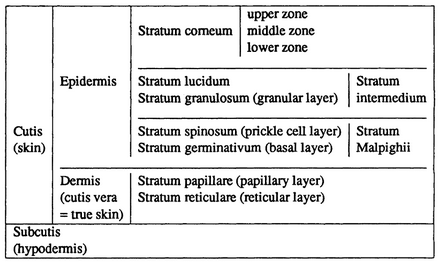
\includegraphics[width=0.8\textwidth]{images/skinLayers.png}
\caption{The Layers of the skin.}
\label{layerTab}
\end{figure}

%epidermis
The epidermis, on its own, can be divided into five different layers and lies on the surface of the skin. It consists of epithelial tissue, which is built in the lowest layer, the stratum germinativum. The main part of the produced cells are keratinocytes, which are able to store keratin and therefore become horny over time. The keratinocytes migrate to the surface of the skin, causing the epidermis to become more horny when approaching the surface. The outer layer is called the stratum corneum, originating from the fully keratinized state of its cells.
On their way to the surface the keratinocytes undergo a number of specific changes in form and areal  distribution, which in part are used to define the different epidermal layers. Also the cells become less tightly packed, compared to the deeper layers, causing the epidermis to become dryer towards the surface. A fact that greatly influences the electrical properties of the epidermis and therefore the  electrodermal activity. The stratum corneum is especially thick in the palmar and plantar regions of the body. Reaching a thickness of approximately 1 $mm$, it is almost 20 times thicker than its overall average of 50 $\mu m$.\\
%dermis
The dermis, which is also referred to as the corium, lies directly beneath the epidermis. Although it is much thicker than the epidermis it is only composed of two different dermal layers, the stratum papillare and the stratum reticulare, which are distinguishable by their density and the arrangement of their collagen fibers. The epidermal dermal junction, which is the transition area between the epidermis and dermis, resembles interlocking hands and is formed by a basal-membrane zone \citep{boucsein2013electrodermal}.
The dermal layer, closest to the epidermis is called the papillary stratum. Other than the capillary net of arterial and venous blood vessels, it contains receptor organs as well as melanocytes and free collagen cells. The second dermal layer, which lies on top of the subcutaneous tissue, is called the reticular stratum. It wears this name because of its texture. Formed of strong collagenous fibers, reticular stratum is highly resistant to rupture, granting the dermis is leathery impression.\\

%subcutis
The subcutis, or hypodermis, is located beneath the dermis and is composed of loose connective tissue. It serves as a connection between the skin and the connective tissue of the muscles, allowing for good horizontal mobility of the skin. The subcutis also serves as a thermal and mechanical insulation layer, due to its ability to store fat. In addition to this it, contains nerves and vessels, which supply the skin with nutrition and information, as well as the hair follicles and secretory part of the glands.   

\begin{figure}[ht]
\centering
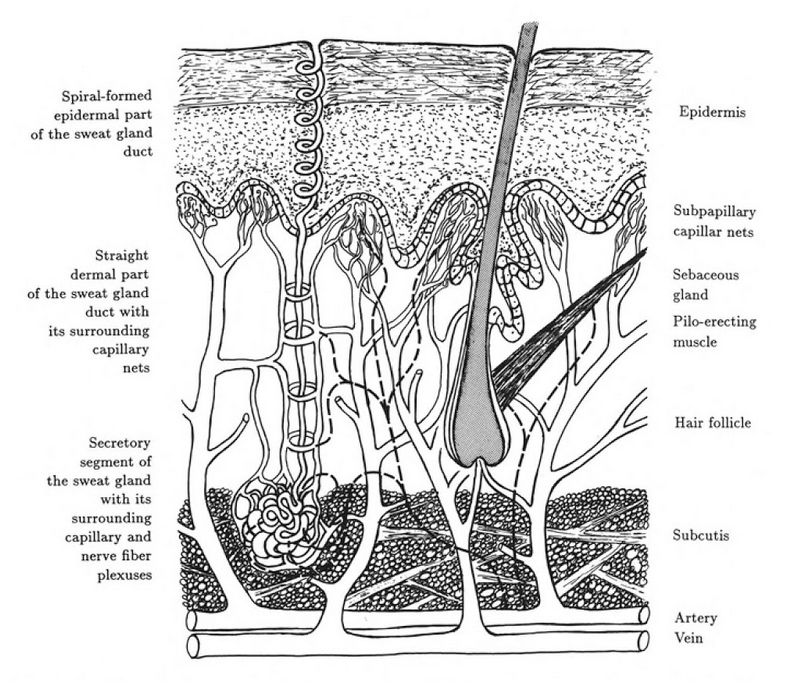
\includegraphics[width=0.7\textwidth]{images/skinDermis.png}
\caption{A artificial cross-section of the skin, combining a sweat gland in ridged skin (left) and a hair together with a sebacous gland in polygonal skin (right).}
\label{DermisImg}
%\citep{boucsein2013electrodermal}
\end{figure} 

%recap link to sweat glands
The left side of figure \ref{DermisImg} shows an example for a typical profile of glabrous (hairless) skin. This specific form of skin differs in its horizontal structure. During early embryonal development specific patterns are formed by ridge formation. Ridged skin can be found on the palms of the hands and the soles of the feet. Areas, both of which, are frequently mechanically stressed and also have been found to have the highest densities of sweat glands, with an average of 233 sweat glands per $cm^{2}$ on the hands and 620 glands per $cm^{2}$ in adult's skin \citep{boucsein2013electrodermal}. Sweat gland are considered to be exocrine glands, which is due to the fact that they secrete directly onto the surface of the skin. There are two types of human sweat glands, eccrine and apocrine, the majority being of the first type. The secretions of eccrine glands only contain negligible amounts of cytoplasm from the glandular cells. As there are no apocrine sweat glands located on the palmar skin, which is the most common location for EDA measurement, this section will only focus on eccrine sweat glands. The main purpose of eccrine sweat glands is to regulate the body temperature. With the exception of the palmar and plantar glands, which are thought to rather take part in grasping behavior \cite{HANDBOOKPP}. Further all eccrine sweat glands are believed to be more responsive to psychologically significant stimuli and therefore to be involved in emotional sweating. Emotional sweating is primarily observable in areas with a high density of eccrine sweat glands, such as hands and feet. Therefore, making these region particularly interesting for EDA measurement, concerning the effect of psychophysiological stimuli. Before elaborating on the connection between electrodermal activity and sweat gland activity, it is useful to consider the anatomy of the glands first.

\begin{figure}[ht]
\centering
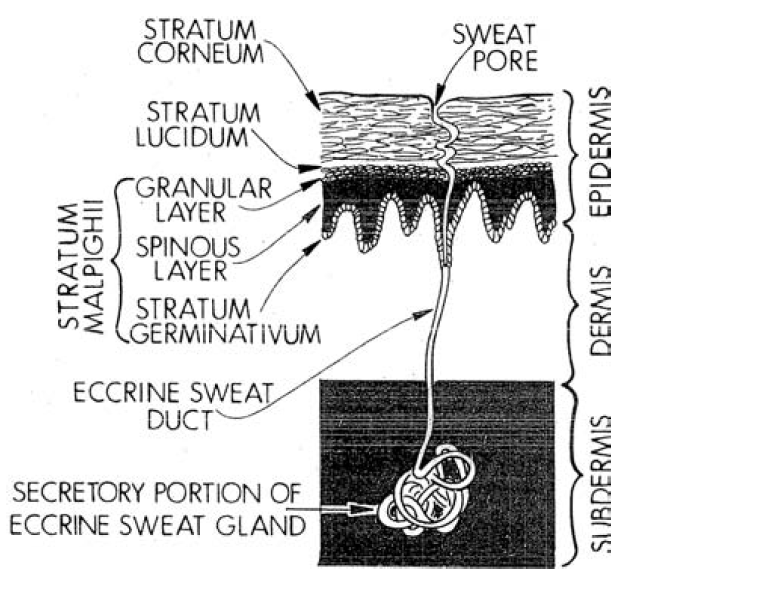
\includegraphics[width=0.7\textwidth]{images/skinAnatomy.png}
\caption{Anatomy of the eccrine sweat gland in various layers of glabrous skin.(Adapted from Hassett, 1978)}
\label{layerImg}
%\citep{HANDBOOKPP}
\end{figure}

Figure \ref{layerImg} shows the anatomy of an eccrine sweat gland in glabrous skin. It consists of the  secretory portion, the coiled compact body of the gland, and the sweat duct. The sweat duct, which is the excretory portion of the gland, is a long tube reaching all the way to the stratum corneum, forming a small pore on the surface of the skin. It passes through the dermis in a relatively straight line but ends up spiraling through the epidermis \cite{HANDBOOKPP}. Imagining sweat glands as a set of variable resistors wired in parallel, helps to understand their influence on electrodermal activity. As sweat rises in the ducts their electrical resistance is constantly reduced, resulting in noticeable changes in electrodermal activity. The amount of sweat and the number of glands that are currently active, and therefore the electrodermal activity depends on the degree of activation of the sympathetic division of the autonomic nervous system.

% innervation
%
%\begin{figure}[ht]
%\centering
%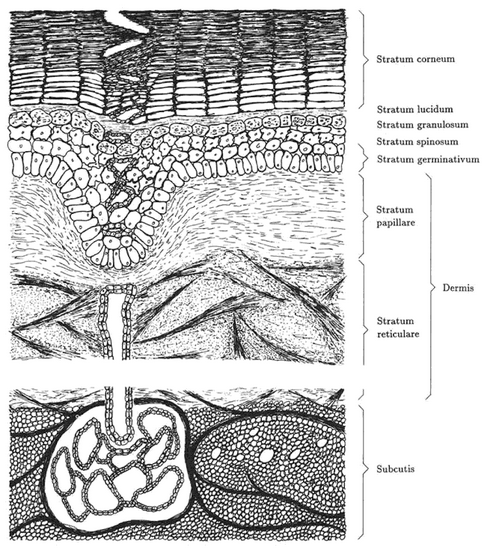
\includegraphics[width=0.7\textwidth]{images/skinGlabrous.png}
%\caption{A cross-section of the layered construction of the glabrous human skin containing an eccrine sweat gland, in its glomerulus, together with its straight dermal and irregularly coiled epidermal duct. A part of the reticular layer has been omitted due to its size in relation to the rest. \citep{boucsein2013electrodermal}}
%\label{glabImg}
%\end{figure}

% physiology
\subsubsection{Physiological basis}
According to the previous section, focusing on the anatomical aspects, this section will outline only the physiological mechanisms required to understand electrodermal mechanisms. 
% efferent innervation of the skin
The autonomic nervous system (ANS) is a complex systems of nerves that regulates involuntary and unconscious actions. The emphasis of this section will be its thermoregulatory aspects, which also involve the skin and sweat glands. 
There are a number of efferent vegetative fibers in the human skin, including sympathetic fibers, innervating the secretory segment of the eccrine sweat glands, and vasoconstrictive efferences for the blood vessels. Originating from the brain, the efferent sympathetic nerves descend in the anterolateral part of the spinal cord in close proximity to the pyramidal tract. They are switched over in the lateral horn and leave the spinal cord through its ventral root. Alongside motoric fibers, the preganglionic sympathetic fibers travel via the white communicating ramus to the sympathetic trunk. From this point the neuronal activity will be distributed to various levels of the sympathetic trunk, causing one preganglionic fiber to reach up to 16 postganglionic neurons. The postganglionic fibers exit the sympathetic trunk through the gray communicating ramus and from there spread into the periphery, eventually reaching the skin.
% sweat gland innervation
Human sweat glands have predominantly sympathetic cholinergic innervation from sudomotor fibers originating in the sympathetic chain. The secretory part of the gland is surrounded by a dense plexus of sympathetic fibers. This allows for a wide distribution of ANS activity. The sudorisecretory fibers form a smooth bundle between the lateral pyramidal tract and the anterolateral tract. They end at the preganglionic sudorisecretory neurons and run right next to the other sympathetic fibers.  Although the sympathetic system is represented in various locations of the brain, the hypothalamus is considered to be the controlling entity of all vegetative functions. This includes sweat secretion and vasomotor activity. However, the central innervation of sweat gland activity is not limited to the hypothalamus. There are several centers, which are located in different levels of the central nervous system and partly independent of one another. The cortex, the basal ganglia, diencephalic structures such as thalamus and hypothalamus, the limbic system and brain stem areas are considered possible origins of sympathetic activity \citep{boucsein2013electrodermal}.

\begin{figure}[ht]
\centering
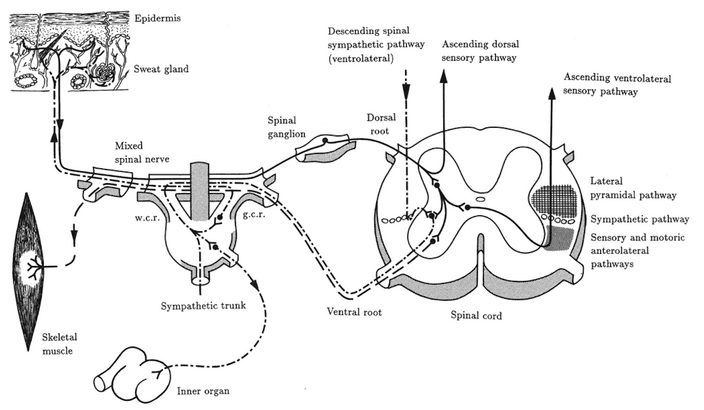
\includegraphics[width=0.7\textwidth]{images/symPathway.png}
\caption{Skin afferents and efferents at spinal cord level and connections with ascending and descending pathways. ---: motoric pathway, -.-: sympathetic efferents. }
\label{symPathImg}
%\citep{boucsein2013electrodermal}
\end{figure}

\subsubsection{Physiology of Electrodermal Activity}
Studies, measuring sympathetic action potentials in peripheral nerves while simultaneously recording EDA, have shown a high correlation between bursts of sympathetic nerve activity and the phasic skin conductance response \cite{HANDBOOKPP}. Because there are many excitatory and inhibitory influences on the sympathetic system, located in various parts of the brain, there also are a variety of neural mechanisms and pathways involved into the central control of EDA.
In a review on CNS elicitation of EDA, Boucsein (2013) concludes that there are two different origins above reticular level: a limbic-hypothalamatic source, which is also thermoregulatory and emotionally influenced, and a premotor-basal ganglia source, eliciting electrodermal concomitants of the preparation of specific motor actions. In addition, Boucsein suggests a third reticular modulating system, mediating EDA changes appearing with variations of general arousal (see figure \ref{znsImg}). Further, an inhibitory EDA system has been located in the bulbar level of the reticular formation.

\begin{figure}[ht]
\centering
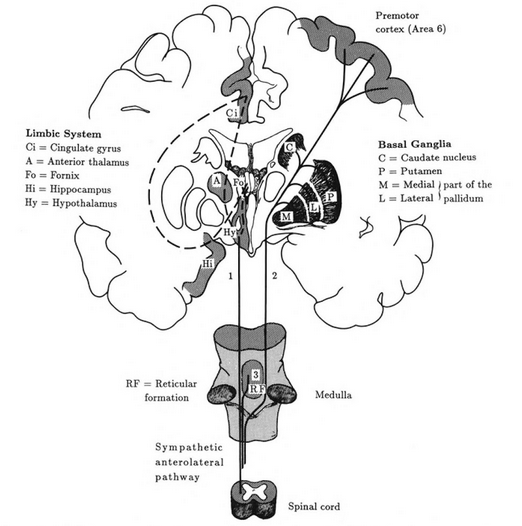
\includegraphics[width=0.8\textwidth]{images/zns.png}
\caption{Central elicitation of EDA in humans. 1: Ipsilateral influences from the limbic system via hypothalamic thermoregulatory areas; 2: Contralateral influences from premotor cortical and basal ganglia areas; 3: Reticular influences. Dashed: Connections within the limbic system.}
\label{znsImg}
%\citep{boucsein2013electrodermal}
\end{figure}

% properties of skin and sweat glands influencing EDA
% eda boucsein 35,36 falls sie mal wieder auftauchen
However, there are also properties of the skin, influencing the EDA, which have to be considered, especially local physiological phenomena related to sweat gland activity. Considering the vertical structure of the skin, there is a significant difference in conductivity between the different layers. Both the dermis and the subcutis are tissues with strong blood supply and interstitial fluid. Therefore their elictrical conductivity is much higher than the conductivity of the epidermal layer, which forms a diffusional as well as an electrical barrier. There has been some discussion concerning the exact localization of an epidermal diffusional barrier, which has been reviewed in detail by Fowles (1986)(see \citep{boucsein2013electrodermal}). However, most of the findings suggest that the entire stratum corneum is forming the barrier, with the exception of its desquamating surface cells\citep{boucsein2013electrodermal}. 
It is to mention that, under normal physiological conditions, the skin temperature is causing changes in permeability of the skin. Fowles (1986) pointed out that the permeability for water doubles with an increase in skin temperature of 7-8  $^{\circ}C$  within the range of 25-39 $^{\circ}C$ (see \citep{boucsein2013electrodermal}). In spite of the diffusional barrier and without activity of the sweat glands, there is always a continuous transmission of water in the skin, directed from the dermis to the outside of the body. This causes the corneum to be always partially hydrated. However, there is a distinct relationship between the relative humidity of the air and the corneal hydration, caused by a dependency of corneal thickness on the relative humidity of the air. As mentioned above there are differences in conductivity in the different skin layers. The barrier, formed by the outer epidermal layers, is penetrated by the sweat gland ducts, which act as diffusional and electrical shunts.
Other than these properties, concerning the resistance, living tissue has capacitative features which are related to the activity of its membranes. While tissue conductivity is mainly responsible for tonic EDA and, in small parts, contributes to phasic electrodermal phenomena with rather slow recovery, active membrane processes following a nerve impulse are prone to eliciting electrodermal responses with fast recovery \citep{boucsein2013electrodermal}.

\subsubsection{Principles of Electrodermal Measurement}
%Currently there are two basic methods of recording, the exosomatic and the endosomatic method. Whereas with the endosomatic method only changes in the potential of the skin are recorded, the exosomatic method relies on an external current to record changes in the skin resistance. This section will focus on the exosomatic method, for it being the current method of choice (Fowles et al.,1981, cited by Cacioppo et al., 2007), and describe the measurement of skin conductance level (SCL) and skin conductance response (SCR), which is the reciprocal of the skin resistance response.\\
%
%Electrodermal activity is measured, by passing a small current through two electrodes, which are placed on the surface of the skin. The physical principal, standing behind this measurement, is Ohm's law. It states that the skin resistance (R) is equal to the voltage (V) applied between to electrodes placed on the surface, divided by the current (I) passing through the skin.
%\begin{center}
%\begin{equation} \label{OhmsLaw}
%R = V/I \qquad ,[R] = \Omega 
%\end{equation}
%\end{center}
%
%There are two concepts to current physiological recording systems. If the current is held constant then the voltage between the two electrodes can be measured. The voltage will vary directly with the skin resistance. Alternatively, if the voltage is held constant the current can be measured. The current will vary directly with the reciprocal of the skin resistance, or skin conductance. The skin conductance is expressed in units of Siemens and measures of skin conductance are usually expressed in units of micro Siemens ($\micro S$). Currently, physiological recording systems that use a constant voltage are the most prevalent for the direct recording of skin conductance.
There are three different methods of measuring EDA: the endosomatic method, which does not rely on the application of an external current, and two exosomatic methods, which apply either direct current or alternating current. For the past couple of decades the measurement of EDA as skin conductance, using a direct current, constant voltage methodology with silver-silver chloride (Ag/AgCL) electrodes and an electrolyte of sodium or potassium chloride has been the most prevalent method in EDA literature \citep{boucsein2012electrodermal}. Thus, the present section will focus on this method. Typically, a small voltage (e.g., 0.5V) is applied to two electrodes, which are placed on the sound surface of the skin, and a small resistor (e.g., 200 to 1000 $\Omega$) is connected in series with the skin.  To avoid any electrocardiogram artifacts, the electrodes should be placed on the same body side. Because the skin resistance exceeds the resistance of the resistor by far, its   effect on the current flow inside the circuit can be neglected, when measuring the current flow. Hence, when applying Ohm's law, the current (I) flow between the electrodes, and therefore through the resistor, is equal to the voltage (U) divided by the Resistance of the skin ($R_{p}$).

\begin{equation} \label{OhmsLaw}
I = U / R_{p}
\end{equation}

Because the voltage has a constant value, the current changes in proportion to the reciprocal of the resistance, which is called conductance ($G_{p}$).  

\begin{equation}
I \approx 1/R_{p} 
\end{equation}
Consequently, the conductance is proportional to the current flow through the skin.
\begin{equation} \label{IG}
I = U \cdot G_{p}
\end{equation}

The unit of conductance is siemens ($S$), where 1 $S$ = 1/1 $\Omega$. According to the skin resistance usually being in the orders of $k\Omega$ or $M\Omega$ , the conductance is very small and often measured in units of $\mu S$. Because the value of the series resistor ($R_{s}$) is constant, the voltage drop across $R_{s}$ is proportional to the current flow I. 

\begin{equation}
U = I \cdot R_{s}
\end{equation}

Considering, the proportionality of I and $G_{p}$, as shown in \ref{IG} it becomes clear that changes in U can be monitored to provide precise index of variations in the skin conductance.\\

\subsubsection{Techniques of Electrodermal Recording}
This section will give a brief overview on possible requirements for electrodermal recording, such as special electrodes, electrode gels and recording devices.

\subsubsection{Electrodes}
Electrodes are a biomedical sensor system. Electrodermal recording typically relies on metal electrodes. However, metal being a generic term, as it is corroded at the surface of the electrode. Different metals will cause different stages of corrosion. Therefore, when measuring EDA with a direct current ,it is of great importance to use two electrodes of the same material, eliminating eventual potential differences. In exosomatic recording, using a direct current, the electrode pair is connected to an external voltage. Thus, turning them into anode and cathode in an electric system, which are polarized by electrolysis.
The standard electrodes, used in electrodermal recording, are sintered silver-silver chloride (Ag/AgCL) electrodes, which minimize both the polarization of the electrode and the bias potential between the electrodes. The most common form of EDA electrodes consist of a metal ring, which is embedded in a cylindrical plastic case. The space between metal and skin is filled with an electrode gel, which usually contains a chloride salt like NaCl. The concentrations of the electrode gel is chosen in the range of 0.050-0.075 molar to resemble the NaCl concentration in human sweat. Therefore, the concentration of the gel will remain stable when mixed with sweat. When using an electrolyte, it is recommended to fix the electrodes to the skin at least 5-10 minutes before starting the recording. This will eliminate an initial  baseline drift in the EDA recording, caused by the electrolyte penetrating the stratum corneum and the sweat ducts. Further the electrode-skin impedance is greatly influenced by the size of the electrolyte-skin contact area and not the size of the electrode metal \citep{boucsein2012electrodermal}. Therefore it is important to give special attention to the electrode fixation, guaranteeing a sufficient electrode-skin contact and a minimization of movement artifacts.

\subsubsection{Recording Sites}
Psychophysiological recordings rely on nonthermoregulatory electrodermal phenomena, which can be most reliably recorded from glabrous skin. Thus making the palms of the hands and the soles of the feet the preferred recording sites for EDA. There are three different ways to place the electrodes when recording EDA on the hand (see Figure \ref{PalmImg}).

\begin{figure}[ht]
\centering
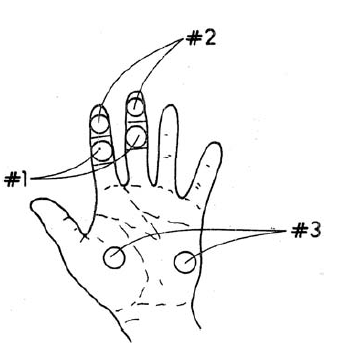
\includegraphics[width=0.5\textwidth]{images/electrodePlacement.png}
\caption{Three electrode placements for recording EDA.}
\label{PalmImg}
\end{figure}

Placement \# 1 involves volar surfaces of medial phalanges, placement \# 2 involves volar surfaces of distal phalanges, and placement \# 3 involves thenar and hypothenar eminences of palms \citep{HANDBOOKPP}.
%It is suggested to place electrodes on the palm of the nondominant hand, presuming it is not as likely to have horny skin. In addition, the placement method \# 2 should be preferred over method \# 1 because of the greater responsivity (Scerbo, Freedman, Raine, Dawson and Venables, 1992, cited by Boucsein et al., 2012) and the greater sweat gland activity of the distal phalanges, compared to the other placement sites(Freedman et al.,1994, cited by Boucsein et al., 2012).\\
It is suggested to place electrodes on the palm of the nondominant hand, presuming it is not as likely to have as much horny skin. In addition, the placement method \# 2 should be preferred over method \# 1 because of the greater responsivity and the greater sweat gland activity of the distal phalanges, compared to the other placement sites \citep{boucsein2012electrodermal}.\\
If both hands are not available for recording, EDA can also be measured at the inner site of the foot , over the abductor hallucis muscle adjacent to the sole and in between the proximal phalanx of the big toe and a point directly beneath the ankle \citep{boucsein2012electrodermal}. In case of exosomatic recording, there is usually no further pretreatment of the skin needed than washing the recording site with warm water.

\subsubsection{Signal Evaluation}
The EDA signal consists of two components, the slow, tonic skin conductance level (SCL) and the faster, phasic skin conductance response (SCR), which need to be addressed separately during the evaluation of the signal.

\subsubsection{Phasic Electrodermal Measures}
Electrodermal responses (EDRs) are short-lasting changes in EDA. They can be elicited by a distinct stimulus or occur without previous stimuli, therefore being called nonspecific EDRs (NS-EDRs). NS-EDRs are considered a tonic measure, meaning they are used to index EDA over a certain time period. In both cases the signal curve follows a certain pattern.

\begin{figure}[ht]
\centering
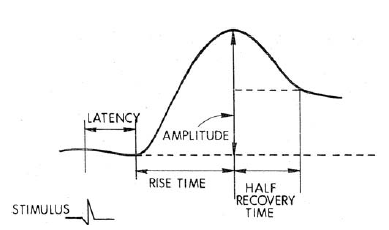
\includegraphics[width=0.7\textwidth]{images/SCR.png}
\caption{Graphical representation of principal EDA components.}
\label{SCRImg}
%\citep{HANDBOOKPP}
\end{figure}

As shown in figure \ref{SCRImg}, there is a characteristic rise from the initial level to a peak, followed by a slower decline. In case of an elicited EDR the time that passes from the stimulus to the onset of the EDR is called latency (EDR lat.), which usually ranges from 1-4 seconds. As pointed out by Boucsein et al. (2012), latencies greater than 4 seconds may occur, but latencies under 1 second should be treated with caution because of system immanent temporal delays, such as time required for stimulus processing, autonomic nervous system nerve conduction to the sweat glands, and penetration of sweat through the ducts to the epidermis. Following the latency, there is an ascent time from the initial level to the peak, which typically varies between 0.5 and 5 seconds \citep{boucsein2012electrodermal}. The peak amplitude (EDR amp.) is reached. To determine the exact value of EDR amp., it is necessary to locate the onset point. Usually, this is done by stepping back along the SCR curve and finding the point of maximum curvature.
%In case of SC measurement, the amplitude is expressed in microsiemens units and is often logarithmically or square-root transformed in order to normalize data.
At times it can be important to determine whether a response has occurred. The occurrence is therefore defined in terms of a minimum amplitude, that has to be reached in order for the event to be counted as a response. This is especially true for NS-EDRs. In the past the threshold value for the minimum amplitude was commonly set to 0.05 $\mu S$. Whereas nowadays, with computerized scoring of EDR records, the definition of the minimum amplitudes has been set as low as 0.01 $\mu S$. It is important to keep in mind, that choosing such a low value might lead to equipment related noise being scored as a response. After the peak deflection, the recovery begins. In this phase the electrodermal reading declines. The recovery is a much slower process than the rise. This is caused by the increase in conductivity of the corneum, elicited by sweat, in the time period following EDRs. There are certain way points, which are usually determined, e.g. the half time recovery (EDR rec.t/2), which is the time that passes until half of the amplitude has recovered. As the recovery proceeds the EDR is concluded.

%show table SCR
\subsubsection{Tonic Electrodermal Measures}
The measures of the relatively long-term tonic EDA states can be divided into two basic principles, the skin conductance level (SCL) and nonspecific skin conductance responses (NS-SCRs). SCL refers to the level of conductance in the absence of phasic SCRs. To guarantee a distortion-free measurement of SCL, all event and artifact related SCRs have to be detected and removed. SCL is typically expressed in units of microsiemens and computed as a mean of several measurements, taken during specific time periods.
NS-SCRs on the other hand are phasic increases in skin conductance that resemble the elicited SCRs. However, they are considered to be tonic components of the EDA signal. The reasoning behind this is the absence of a distinct stimulus, related to their occurrence. According to SCL, NS-SCRs can be recording in periods without or in between a stimulus presentation, e.g. a resting phase. NS-SCRs usually are expressed in number of responses per time interval, most commonly per minute. As mentioned before it is important to define a threshold to determine which responses will be rated as such.

\subsubsection{Psychological and Social Context of EDA}
%SCL and NS-SCRs have been widely used as indices of sympathetic nervous system arousal.
This section is based on a review of the psychological an social factors that have been shown to influence EDA, done by Cacioppo et al. (2007). Three different types of paradigm have been reviewed: (1) those that involve the presentation of discrete stimuli, (2) those that involve the presentation of continuous stimuli, and (3) those that involve examining the correlates of individual differences in EDA. The present section will briefly cover the first two types.

\subsubsection{Effects of discrete stimuli} 
There are a number of stimuli attributes to which the SCR is sensitive, including stimulus novelty, arousal content, significance, intensity and surprise. Although it may be impossible to identify an isolated SCR as an "attentional" response or an "anxiety" response, it is however possible, to interpret the psychological meaning of a SCR by providing a strict experimental paradigm. The better controlled the experimental paradigm, the more conclusive the interpretation. If there is only one attribute of the stimuli changing during the experiment, such as intensity, elicited SCRs can be matched more precisely and therefor allow a better interpretation of the psychological process involved. For example, the International Affective Picture System (IAPS), which has been developed by Lang et al. (1998), consists of a variety of pictures that are rated for both their arousal-producing quality and their valence. The valence scale ranges from strongly positive to strongly negative pictures. SCRs elicited by the use of the IAPS have been found to be related to the arousal dimension, with responses increasing  in magnitude as arousal rating increased for both positively valenced and negatively valenced pictures \cite{HANDBOOKPP}.

\subsubsection{Effects of continuous stimuli} 
In contrast to the brief, discrete stimuli, as reviewed earlier, continuous stimuli are rather long-lasting and can be thought of as modulating changes in tonic arousal. In this context SCL and the frequency of NS-SCRs provide the most useful measures of EDA, because they can be measured over long periods of time. There are certain continuous stimulus situation which will reliably produce an increase in EDA. One example that can be mentioned here is performing a task. Performing as well as anticipating almost any task will cause an increase of both SCL and the NS-SCR frequency. This has already been shown by the following studies, which have been reviewed by Caciappo et al. (2007). Lacey et al. (1963) recorded palmar SCL during rest and during anticipation and performance of eight different tasks. They confirmed an increase of SCL in every task situation. According to the results the SCL rose by one $\mu S$ during anticipation and by another one or two $\mu S$ during performance, when compared to the resting level. Other findings suggest that situations in which strong emotions are elicited also increase tonic EDA arousal. Ax(1953) created genuine states of fear and anger in his subjects by causing them to believe to feel in danger of a high-voltage shock due to equipment malfunction or by treating them in a rude fashion. Both SCL and NS-SCRs rose during the fear as well as the anger conditions \cite{HANDBOOKPP}. 

% evtl conclusion
% EPILOGUE
%EDA is a sensitive peripheral index of sympathetic nervous
%system activity that has proven to be a useful psychophysiological
%tool with wide applicability. Social and behavioral
%scientists have found that tonic EDA is useful to investigate
%general states of arousal and/or alertness, and that the
%phasic SCR is useful to study multifaceted attentional processes,
%as well as individual differences in both the normal
%and abnormal spectrum ( zitat aus Cacioppo 2007)
\subsubsection{Conclusion}
In conclusion, EDA serves as a sensitive peripheral index of sympathetic nervous system activity. As mentioned above, the eccrine sweat glands are entirely under sympathetic control and therefore increases in both SCL and SCR mirror tonic and phasic sympathetic activation. EDA provides for a relatively direct and inexpensive measure that comes with great utility and can be used as an reliable indicator of arousal and attention.
\newpage

\subsection{Electrocardiogram}

\subsubsection{Anatomical and Physiological Basis}
The cardiovascular system consists of two main components, the heart, which functions as a pump, and the vasculature, as a distribution system, that together ensure a constant blood supply throughout the whole body. The heart provides a steady flow of oxygenated blood, by sending blood into the lungs (pulmonary circulation) and then to the rest of the body (systemic circulation).

\begin{figure}[ht]
\centering
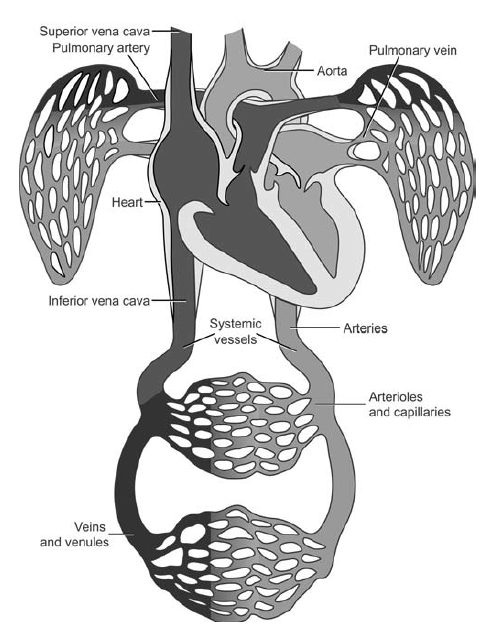
\includegraphics[width=0.7\textwidth]{images/CVS.png}
\caption{Ventral perspective of the systemic and pulmonary circulation. Lighter gray areas indicate oxygenated blood and darker gray areas indicate deoxygenated blood.}
\label{CVSImg}
%\citep{HANDBOOKPP}
\end{figure}

As can be seen on figure \ref{CVSImg} the deoxygenated blood returns to the heart through the superior and inferior vena cava. After passing the right atrium the venous blood reaches the right ventricle of the heart, from where it is pumped into the lungs for re-oxygenation purposes. Completing the pulmonary circulation, the oxygenated blood returns to the heart through pulmonary veins, reaching the left atrium first and finally the left ventricle. From here the blood is pumped into the aorta and distributed in the rest of the body. On its way to the periphery the blood passes through ever smaller vessels, starting with large arteries, which later branch into smaller arterioles and finally into capillaries. The capillaries are small, thin walled vessels from which oxygen, nutrients and waste products, such as carbon dioxide, are exchanged with the tissue. Leaving the capillaries, the blood returns to the heart again through the venous part of the systemic circulation. After passing the slightly larger venules the blood flows into increasingly larger veins until it reaches the vena cava and the circle closes.\\
The human heart can be divided into four chambers, two on either side. Each of the sides consists of an atrium at the top, or rostral, half and a ventricle at the bottom, or caudal, half. The heart contains three different types of cardiac muscle tissue, atrial and ventricular muscle fibers as well as specialized conducting fibers. The muscle fibers primarily serve the pumping function of the heart but also form a syncytium. This means, the tissue is electrically coupled in a way that allows for a rapid spread of depolarization along the longitudinal axis of the heart. There are two separate syncytiums, the atrial and the ventricular one, which are connected by an electrical conducting system. Although they are electrically connected it is crucial that both portions of the heart function as separate pumping units and all chambers are coordinated, in a way where the ventricular action is always triggered shortly after the atrial action.\\
This challenge is met by a special conducting system, formed out of specialized conducting fibers, which is embedded into the cardiac muscle tissue. The contraction of the heart can be triggered by the depolarization of two nodes of electrically active tissue, the first one being the sinoatrial (SA) node followed by the atrioventricular (AV) node. The SA node, serves as the pacemaker of the heart and is located inside the wall of the right atrium right beneath the entering point of the vena cava superior.  
%"The SA node is the pacemaker because the speed of spontaneous depolarization of this node is typically faster than that of the AV node, and hence generally controls the rate of the beat" HandbookPP
A system of internodal, conductive fibers connects the two nodes. The depolarization wave is transported into the ventricles by passing the bundle of His, which branches into the left and right bundles and then transition into the Purkinje fibers. These fibers pass through the interventricular septum and deliver the depolarization into the rest of the ventricles.\\
The cardiac cycle is a term that describes all events that occur in the heart from one beat to the next (see figure \ref{cycleImg}). The cycle is divided into two main phases, the diastole and systole. During the systole the pumps and the blood is evacuated into the arteries, whereas the heart will be filled again during the diastole. The electrocardiogram (ECG) is the graphical representation of the electrical potential produced by the electrical current passing through the heart. It is recorded via electrodes positioned on the body surface and displayed in forms of so called waves or deflections \cite{ABDULLA2014}.

\begin{figure}[ht]
\centering
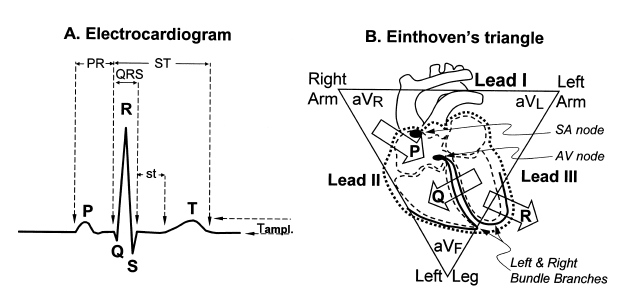
\includegraphics[width=0.7\textwidth]{images/ecg.png}
\caption{A: General morphology of the ECG showing P, Q, R, S, and T components, the PR, ST and QRS intervals, the st segment, and the T wave amplitude; B: The heart, conducting system, and Einthoven's triangle. Open arrows indicate the direction of propagation of electrical activation and the associated component of the ECG.}
\label{ecgImg}
%\citep{HANDBOOKPP}
\end{figure}

The cycle starts with the depolarization of the SA node during the final stage of the diastole. The process of the depolarization wave passing through the atrial muscle tissue corresponds to the P wave of the ECG. Following the P wave is the atrial contraction, during which the QRS complex appears in the ECG. This complex reflects the contraction of the ventricles and the demarcation of the onset of the systole. During the contraction, the intraventricular pressure reaches levels high enough to close the AV valves, which are located between the atria and the ventricles. After the ventricular contraction has ended the ventricular pressure will start to drop again, eventually causing it to fall below the atrial pressure and allowing the AV valves to open and the blood to fill the ventricles. However, once the the ventricular pressure exceeds the aortic pressure the aortic valve opens and blood is evacuated into the systemic circulation. In the latter part of the ventricular contraction phase the ventricles repolarize, creating the T wave in the ECG and initiating the relaxation of the ventricles as well as the onset of diastole. 

\begin{figure}[ht]
\centering
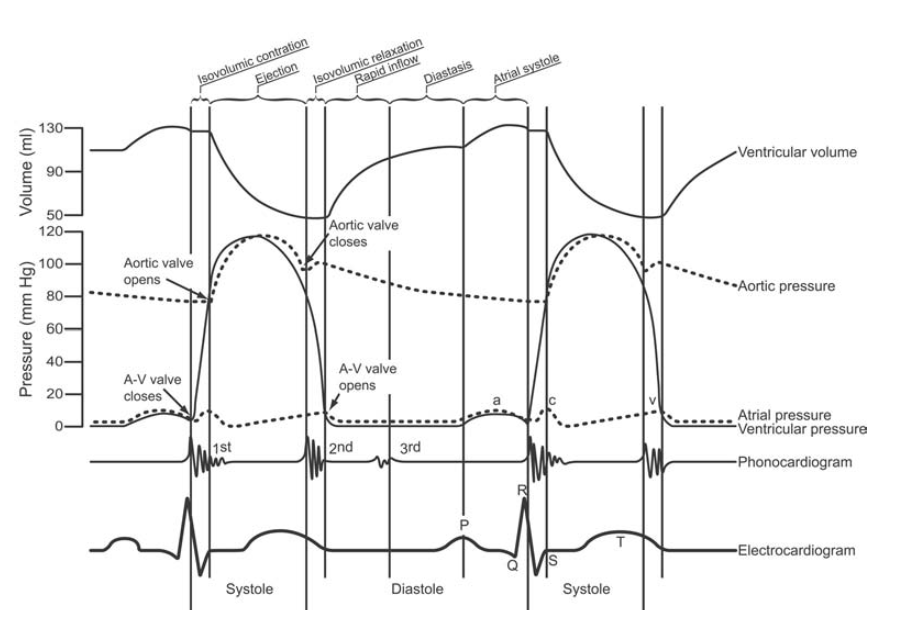
\includegraphics[width=0.9\textwidth]{images/cycleImg.png}
\caption{The graphic shows two full cardiac cylces for various aspects, which can be seen on the right.}
\label{cycleImg}
%\citep{HANDBOOKPP}
\end{figure}

%\subsubsection{Autonomic control}
%The cardiovascular system is under the control of both branches of the autonomic nervous system, the sympathetic and the parasympathetic branch.

\subsubsection{ECG Measurement}
As mentioned above, the ECG is a graph that represents cardiac electrical activity from one instant to another. The ECG pictures the heartbeat in the form of a time-voltage chart. The general study of ECGs, including its clinical applications and technological aspects, is called electrocardiography \cite{GOLDBERGER2017}. Accordingly, the device, used to measure and display the conventional (12-lead) ECG, is called an electrocardiograph. It records the cardiac electrical activity through electrodes, which are positioned selectively on the body surface. Current ECGs most commonly use disposable self-adhesive silver-silver chloride electrodes, which were traditionally placed on the limbs. These extremity leads can be represented by the Einthoven triangle (see Figure \ref{ecgImg}B). As illustrated there are six leads in total, three unipolar leads, which are taken of the right arm ($aV_{R}$), the left arm ($aV_{L}$) and the left leg ($aV_{F}$), as well as three bipolar leads, taken between I: left arm - right arm, II: left leg - right arm and III: left leg -left arm, with the right leg being the ground. Typically these leads are approximated by placing the electrodes on the torso instead of the limbs. In clinical cardiology, a series of unipolar precordial chest leads are usually added to provide a variety of distinct electrical perspectives on certain heart events. These leads start from the right lower peristernal region, with the first lead being labeled V1, and extend laterally to the left (V2-V6). However, for most psychophysiological applications a simpler configuration, such as lead II, will suffice as they still yield a large enough R wave \citep{HANDBOOKPP}. 
%The amplitude of the T wave (see Figure 8.3A) has been
%proposed as a measure of sympathetic control of the heart,
%as it is sensitive to sympathetic activation or beta adrenergic
%drugs, but less so to cholinergic drugs or markers
%of parasympathetic activity (see Contrada, 1992; Furedy,
%Heslegrave, & Scher, 1992; Kline, Ginsburg, & Johnston,
%1998). This measure has not received general acceptance,
%however, as it does show some sensitivity to cholinergic
%manipulations (Annila, Yli-Hankala, & Lindgren, 1994),
%and shows inherent rate dependent changes (Contrada,
%1992; Kline et al., 1998) that are independent of, and can
%be as large as, autonomic effects (Rashba et al., 2002).

\subsubsection{ECG Signal Components}
The present section is based on the work of Goldberger et al. (2017) and will briefly outline all components of an ECG signal. The clinical ECG graph consists of three different component types, waveforms, intervals and segments. Their distribution is specified by the 5-4-3 rule, which states that there are five waveforms (P, QRS, ST, T and U), four sets of intervals (PR, QRS, QT/QTc and RR/PP) and three segments (PR, ST and TP)\cite{GOLDBERGER2017}.

\begin{figure}[ht]
\centering
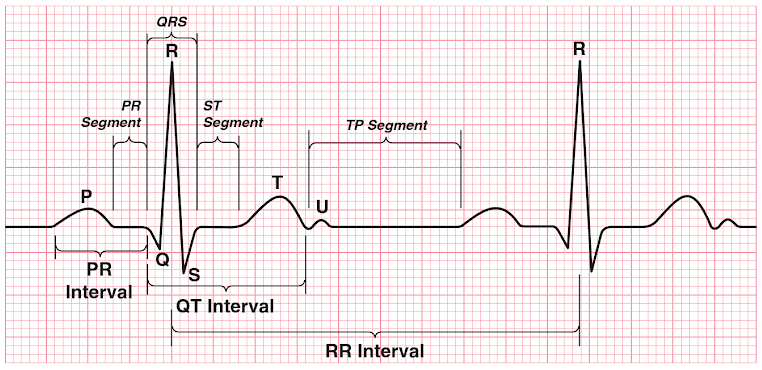
\includegraphics[width=0.9\textwidth]{images/ecgcomp.png}
\caption{Summary of all major components of the ECG graph.}
\label{ecgcompImg}
%\citep{GOLDBERGER2017}
\end{figure}

\textbf{Waveforms}\\ 
The five basic ECG waveforms are named alphabetically, starting with the P wave, which represents atrial depolarization. The QRS waveform, which is often referred to as QRS complex, represents the ventricular depolarization. The ST and T wave represent the ventricular repolarization, eventually resulting in the U wave depicting the final stage of said repolarization. The atrial repolarization is generally not observed, because of the small amplitudes of the atrial ST segment and atrial T wave. Together these waveforms represent a complete cycle of the electrical activity of the heartbeat.\\

\textbf{Segments}\\ 
As mentioned before there are three basic segments contained in the ECG graph, which are defined as the spaces between two waveforms. The PR segment is defined as the distance between the end of the P wave and the start of the QRS complex. It marks the start of atrial repolarization, which is continued throughout the QRS complex and ending during the ST segment. The ST segment spreads from the end of the QRS complex to the beginning of the T wave. TP segment connects the end of the T wave with the beginning of the P wave of the next cycle. This segment represents the electrical resting state and is typically used as a baseline reference for PR and ST deviation assessment in clinical diagnostics.\\

\textbf{Intervals}\\
 Per definition intervals are parts of the ECG that include a minimum of one entire waveform. The PR interval is measured from the beginning of the P wave to the beginning of the QRS complex and is followed by the QRS interval, which lasts until the end of the same QRS complex. The QT interval is defined from the start of the QRS complex to the end of the T wave. The RR interval is the last of the four and lasts for an entire heart cycle, starting and ending at a predefined point in the QRS complex, which is often referred to as the R point. It can be used to calculate the instantaneous heart rate (HRi) in the following manor.

\begin{equation}
HRi = 60 / RR \qquad \text{,RR in units of seconds}	
\end{equation}

\subsubsection{Heart Rate and Heart Period}
The heart period (HP) is the time in milliseconds between two heart beats. It is usually determined by measuring the distance between to successive R spikes in an ECG, due to their prominence in comparison to the other components. The heart rate (HR) is a more common way when communicating heart activity. Typically the heart rate is given in beats per minute (bpm) and can be determined by calculating the reciprocal of the heart period.

\begin{equation}
HR = 60000 / HP
\end{equation}

There are incidents however, in which heart rate and period are not linear. As mentioned by Caciappo et al. (2007) "Berntson and colleagues (1995) reviewed literature across several mammalian species, including humans, showing that the relationship between changes in activity of the parasympathetic and sympathetic autonomic branches and heart period are more nearly linear than the relationship between activity in either branch and heart rate". This means that certain change in activation of either branch of the ANS will result in an equal change in heart period, whereas the same is not true for heart rate. It is important to mention that the change in heart period is independent from the baseline heart period at the time. For example,  raising the stimulation frequency of the vagal nerve by 2 Hz in dogs, results in a change of 70-72 msec in heart period, regardless of the baseline heart period being either 875 msec or 350 msec. In contrast, applying a 2 Hz change in parasympathetic activation resulted in different heart rate changes for either baseline. Heart rate of dogs with a heart period baseline of 875 msec changed by 5.1 bpm and by 29.2 bpm for a 350 msec baseline \citep{HANDBOOKPP}. Therefore the choice of the metric can heavily influence the outcome of an experiment. Bernston et al. (1995) recommended heart rate as the metric of choice when changes in cardiac functions are likely to be caused by autonomic effects and when those changes vary widely as a result of an experimental manipulation or between groups because errors caused by the nonlinear relationship between autonomic inputs and heart rate can be significant and result in misinterpretations of the data \citep{HANDBOOKPP}.

\subsubsection{Heart Rate Variability}
The oscillation in the interval between consecutive heart beats as well as the oscillation between consecutive instantaneous heart rates is called heart rate variability (HRV)(Task Force of the European Society of Cardiology the North American Society of Pacing Electrophysiology, 1996 ; from now on Task Force).
Measures of the HRV can be divided into three general groups, the time domain methods, the frequency domain methods and non-linear methods. Time based methods determine either the HR at any given point in time, by calculating the HRi, or the intervals between successive normal complexes, by detecting the so called normal-to-normal (NN) intervals.
Simple time–domain variables that can be calculated include the mean NN interval, the mean heart rate and the
difference between the longest and shortest NN interval(Task Force, 1996). Frequency domain methods on the other hand decompose the overall heart period variance into specifiable frequency bands \citep{HANDBOOKPP}. A common approach are power spectral density (PSD) analysis, which are based on a Fast Fourier Transform (FFT) of the HRV and provide basic information on how power distributes as a function of frequency. When considering only short time HRV recordings ranging from 2 to 5 minutes three major spectral components can be distinguished. There are very low frequency (VLF), low frequency (LF) and high frequency (HF) components \cite{TASK1996}. The distribution of the power and the central frequency of each frequency band vary in regard to changes in autonomic modulation of the heart period. In general high-frequency HRV is mostly attributable to variations in the parasympathetic control associated with respiration and is commonly used as an index of vagal control of the heart \citep{HANDBOOKPP}. Whereas low-frequency HRV's psychological significance remains a controversial topic. Contrary to the assumption of LF HRV being related to cardiac sympathetic activity it seems to rather  reflect both sympathetic and vagal influences related to baroreflex mechanisms \cite{BERNTSON1997}.

Non-linear phenomena are determined by a number of complex interactions of haemodynamic, electrophysiological and humoral variables, as well as autonomic and central nervous regulations \cite{TASK1996}. Although a  variety of techniques has been applied to determine non-linear properties no major breakthrough in the field of HRV analysis has been achieved yet. 

\section{General}
\subsection{Related Work}
Virtual reality combines real-time computer graphics, body-tracking devices and high-resolution visual displays to create a computer-generated virtual environment. With their ability to immerse the user into a virtual mirror of the real world, virtual environments are a powerful tool in clinical application, especially in the treatment of phobias \cite{RIVA2003}. \\
Studies have shown anxiety disorders to be the most prevalent mental disorders \cite{KESSLER2005}. Many consider exposure therapy the most effective form of treatment for specific phobias \cite{DERUBEIS1998}. However that may be, considering the nature of certain phobias, such as fear of heights, exposure therapy involves a genuine risk of injury. Performing therapy in a virtual environment therefore can be a promising alternative to the conventional in-vivo exposure.\\ 
The efficacy of virtual reality exposure therapy (VRET) has already been demonstrated in the past. A study conducted on acrophobia compared two groups of student subjects. The first group received a graded VRET. Whereas students of the second group were added to a waiting-list as a control group. Results showed VRET to be more effective than no treatment \cite{ROTHBAUM1995}. A few years later, VRET was also found to be as effective as exposure in-vivo in a more recent work by Emmelkamp et al. (2002).\\
In addition to this using a virtual reality system can have a number of advantages over in-vivo exposure. First and foremost being the ability to conduct therapy inside a controlled and secure environment like a therapist's office for example. This also implies therapy being less time consuming and provides considerable financial benefits \cite{CAVANAGH2004}. The possibility of having therapy in a more private scenario also increases the likelihood of acceptance in people that are too anxious or afraid of public embarrassment. 
A recent study exploring the acceptability of virtual reality exposure and in-vivo exposure in subjects suffering from specific phobias supports this hypothesis. When given the choice, 76\% of the subjects chose virtual reality exposure over in-vivo exposure. In addition to this the refusal rate of 3\% for virtual reality exposure was substantially lower than 27\% for in-vivo exposure \cite{GARCIA2007}. Further epidemiological studies have shown a lifetime prevalence of 28.5\% for vHI and 6.4\% for acrophobia alone and that only 11\% of susceptible people were willing to consult a doctor \cite{HUPPERT2013} \cite{KAPFHAMMER2015}.\\
These results illustrate just how difficult and intimidating an in-vivo exposure can be to a phobic and how virtual reality exposure could help increase the number of people who seek therapy for phobias and therefore needs to be established in everyday clinical work.\\
In recent years there has been a lot of research on virtual reality treatment for different phobias trying just that.\\
For example a controlled study by Rothbaum et al. on aerophobia (2000) as well as an open clinical trial on post-traumatic stress disorder (2001) and a study on agoraphobia by Meyerbröker et al. (2011), all of which yielded positive results \cite{ROTHBAUM2000} \cite{ROTHBAUM2001} \cite{MEYER2011}.
Aside from these studies researching the general use of VRET, there also have been studies on ways to control the virtual reality. In a pilot study, Levy et al. (2016) explored the possibility of a remote-controlled virtual reality. After a trial session in a neutral virtual environment the patients received a total of six therapy sessions. The first three sessions were remote-controlled virtual reality exposure therapy (e-VRET) followed by three sessions in the presence of a therapist (p-VRET). E-VRET sessions were conducted without any contact to the hospital staff. The study showed that e-VRET not only is possible but produces results equal to p-VRET \cite{LEVY2016}. This inevitably leads us to the idea of a entirely independent VRET, which to some degree already exist on the market. This is an idea of which we shy away from. In regard to the possible harm that could be caused by patients attempting to treat themselves instead of a receiving professional consultation.
Assessing the mental state of a patient is essential for the success of the therapy. A task which usually falls to the hands of the psychiatrist, leading the exposure, and in most cases relies on a verbal communication between both parties.
Returning to the topic of an e-VRET, intending to ensure the quality of our system we clearly have to provide some sort of substitute for this.\\
Past studies have shown a strong psychophysiological arousal in in-vivo exposure for different specific phobias \cite{NESSE1985} \cite{ALPERS2007}. In a more recent work Diemer et al. (2015) also confirmed physiological arousal in subjects executing a virtual height challenge \cite{DIEMER2016}. The study examined phobics and healthy controls in terms of subjective and physiological fear reactions resulting in a significant increase of subjective fear, heart rate and skin conductance level. 
Emmelkamp et al. (2001) also used psychophysiological measures to actively guide the therapy. To aid the therapist in deciding whether anxiety had diminished, the heart rate was monitored throughout the virtual reality exposure sessions using an ambulatory heart rate device. The actual heart rate was displayed continuously on a monitor. Based on reduction in the subjects subjective anxiety rating and heart rate, the therapist could decide to switch to an exposure scene with higher difficulty \cite{EMMELKAMP2001}. This method was found to be very well accepted by the therapists, for compensating the patient's low ability of introspection when experiencing anxiety or a panic attack. 
In conclusion, virtual reality exposure is a valid alternative to in-vivo exposure and can be used to efficiently treat people suffering from phobias, especially when paired with psychophysiological measurement.
%We base our hypothesis on these results and claim a virtual reality system, relying on real-time measurement of changes in heart rate and skin conductance paired with an adaptable virtual environment, can simplify treatment and improve the quality of VRET.\\
%The present thesis is prior to a study in cooperation with the psychiatry department of the University Hospital Saarland concerning VRET on acrophobia.
 
%To prove this hypothesis, we designed a virtual environment for the treatment of acrophobia that is sufficiently adaptable to various degrees of acrophobia. We will show the effectiveness of our system based on a subjective rating as well as heart rate and skin conductance measurements. Further we will deploy our virtual environment in a closed loop virtual reality system, featuring multiple control units. We will conduct a experiment simulating the effect of real-time physiology based decision making by using a remote-controlled virtual reality.\\

\subsection{Problem Analysis and Goals}
%- analyze the problem with current models of exposure therapy
%- show that my approach is different and how
%- why my approach is better and makes sense
%- goal is a safe and effective therapy option for acrophobia
In this section we will have a closer look at the preceding studies on phobia treatment, analyzing methods and show ways of improvement.
There are two major conditions, which have to be met for an exposure therapy to be successful. The first condition is the ability to elicit fear in the patient. A task that as has been shown can be achieved by a number of virtual scenarios. However, past virtual reality environments exclusively featured either a single stimulus strength, a number of scenes with different stimuli, which required the user to change scenes in order to alter the difficulty of the exposure, and exposure scenarios with varying difficulty, which were presented in a certain routine. These methods may be sufficient for research purposes but to integrate them into actual therapy some alterations have to be made. For example, to fit the needs of a variety of patients, a virtual height challenge with only one intensity is highly insufficient. Whereas on the other hand a monotonous experience is unlikely to maintain a certain degree of activation over a number of sessions. In addition, frequent changes in scene will hurt the immersion of the patient and therefore might interfere with the treatment. In consideration of these arguments our goal was to design a virtual environment that features a progressive and seamless transition between a variety difficulties, and real-time adaption to the current needs of both patient and therapist. The second condition for a successful therapy is to allow for emotional processing (see \ref{EXPEP}). This means that the effectiveness of the treatment is closely related to the fact how the patient perceives information during the exposure. It is necessary for the exposure to be long enough so the patient can habituate to the situation an receive corrective information. Thus, to optimize exposure time we provide the will provide the therapist with a steady stream of information in the form of a graphical presentation of skin conductance and heart rate variance. Our goal is to provide a system that features a closed loop of constant information flow.


%Therefore we have designed a virtual reality environment, in which patients are confronted with a virtual height challenge, centered around a descending floor in an otherwise non-stimulating room. This situation is, in a way, an inverse version of the commonly used elevator scenario. We have chosen this variant to eliminate the reduction in immersion that can be caused by the missing sensation of the elevator movement.

